	% 代码分析:模块功能、涉及到的类、类关系、数据结构及关键代码等;
	% 任务要求,设计任务要求;
	% 设计:详细的设计方案,相关的数据结构、算法描述,可采用伪代码等形式化描述
	% 实现:修改哪些类、如何修改、为什么修改等;
	% 测试:测试用例,测试结果及结果分析,测试运行界面等;
	% 调试:调试方法,遇到的问题及解决方案等;
	% 结论与展望:完成的主要工作、收获、进一步的工作,建议、体会、心得等;

\section{作业1}
\subsection{作业1.1}
\subsubsection{题目描述}
画图表示编译过程的各个阶段,并简要说明各阶段的功能。

\subsubsection{解答}
\begin{figure}[H]
    \centering
    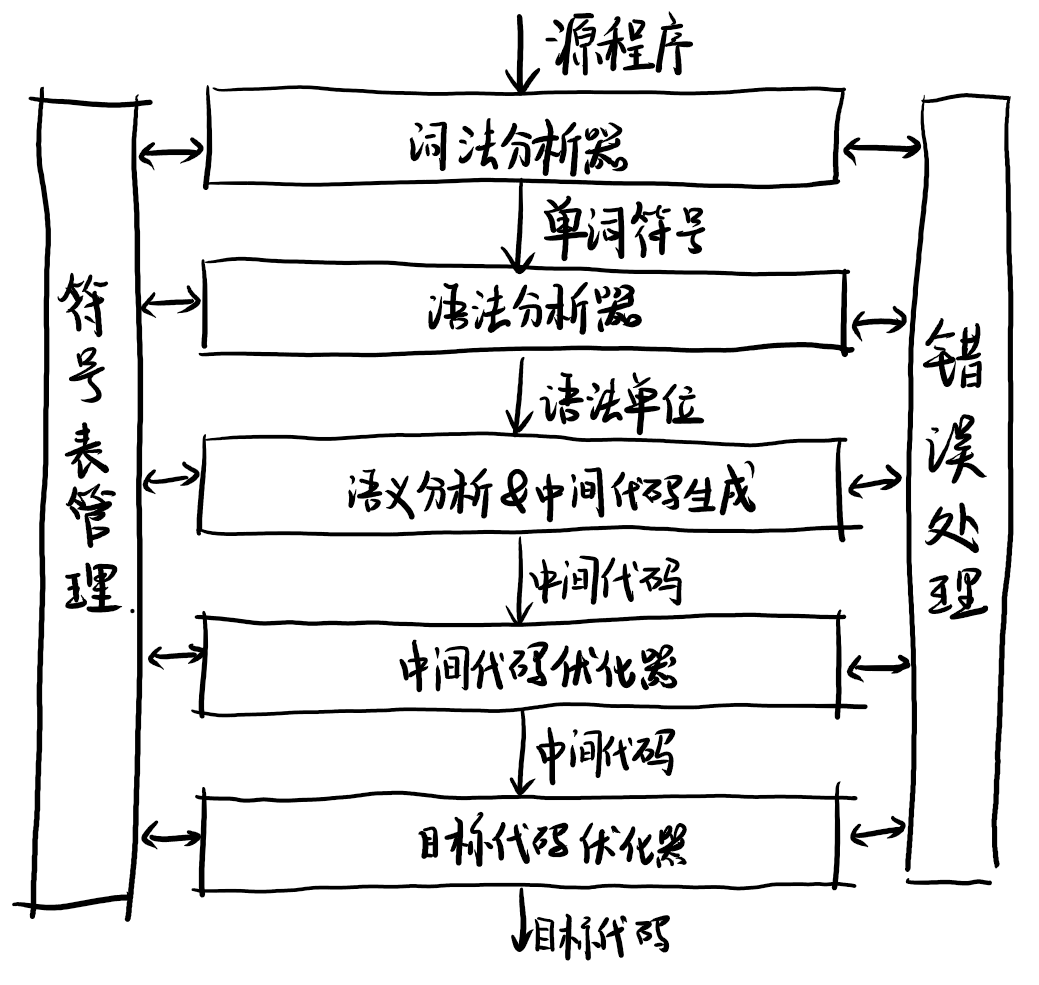
\includegraphics[width=0.6\linewidth]{imgs/编译过程.png}
    \caption{编译过程的阶段}
    \label{fig:编译过程阶段}
\end{figure}

\begin{enumerate}
\item \textbf{词法分析器}:又称扫描器,输入源程序,进行词法分析,输出单词符号。
\item \textbf{语法分析器}:又称扫描器,对单词符号串进行语法分析,识别出各类语法单位,最终判断输入串是否构成语法上正确的“程序”。
\item \textbf{语义分析与中间代码生成}:按照语义规则对语法分析器归约(或推导)出的语法单位进行语义分析,并把它们翻译成一定形式的中间代码。
\item \textbf{中间代码优化器}:对中间代码进行优化处理。
\item \textbf{目标代码生成器}:把中间代码翻译成目标代码。
\item \textbf{错误处理}:发现各种错误、准确指出错误的性质和发生错误的地点、将错误所造成的影响限制在尽可能小的范围、自动校正错误(如果可能)。
\item \textbf{符号表}:用于登记源程序的各类信息和编译各阶段的进展状况。
\end{enumerate}

\subsection{作业1.2}
\subsubsection{题目描述}
求表达式 “$a \vee b \neq c+d \land a * b<f$” 的后缀式。
\subsubsection{解答}
\begin{table}[h]
\centering
\begin{tabular}{>{\centering\arraybackslash}m{3cm}>{\centering\arraybackslash}m{3cm}>{\centering\arraybackslash}m{4cm}>{\centering\arraybackslash}m{3cm}}
\toprule
\textbf{类别} & \textbf{算符} & \textbf{符号} & \textbf{结合性} \\
\midrule
位运算符 & 按位取反 & $\sim$ & 右结合 \\
\midrule
\multirow{3}{*}{算术算符} & 幂、负 & $**, -(@)$ & 右结合 \\
\cmidrule{2-4}
 & 乘除、取余 & $* (\times), /(\div), \%$ & 左结合 \\
\cmidrule{2-4}
 & 加减 & $+, -$ & 左结合 \\
\midrule
位运算符 & 左移、右移 & $\ll, \gg$ & 左结合 \\
\midrule
\multirow{2}{*}{关系算符} & 大于小于 & $<,\leq, >,\geq$ & 不可结合 \\
\cmidrule{2-4}
 & 等于不等 & $=, \neq$ & 不可结合 \\
\midrule
\multirow{3}{*}{位运算符} & 按位与 & $\&$ & 左结合 \\
\cmidrule{2-4}
 & 按位异或 & $\oplus$ & 左结合 \\
\cmidrule{2-4}
 & 按位或 & $|$ & 左结合 \\
\midrule
\multirow{3}{*}{逻辑算符} & 非 & $\neg , !, \text{或 \textbf{not}}$ & 右结合 \\
\cmidrule{2-4}
 & 与 & $\land ,\&\&, \text{或 \textbf{and}}$ & 左结合 \\
\cmidrule{2-4}
 & 或 & $\lor ,||, \text{或 \textbf{or}}$ & 左结合 \\
\midrule
三目算符 & 三目算符 & $?$ : & 右结合 \\
\midrule
赋值算符 & 赋值等 & $= \text{或 :=}$ & 右结合 \\
\bottomrule
\end{tabular}
\end{table}
按照算符优先级,有:
\begin{align*}
& {\color{Red} <}  a \vee b \neq c+d \land a * b<f{\color{Red} >}  \\
= & {\color{Red} <}  a{\color{Red} >} {\color{Red} <} b \neq c+d \land a * b<f{\color{Red} >} \vee\\
= & a {\color{Red} <} b \neq c+d {\color{Red} >}{\color{Red} <} a * b<f{\color{Red} >}\land \vee\\
= & a{\color{Red} <} b{\color{Red} >} {\color{Red} <}c+d{\color{Red} >}\neq{\color{Red} <} a * b{\color{Red} >}{\color{Red} <}f{\color{Red} >}<\land \vee\\
= & abcd+\neq ab*f<\land \vee
\end{align*}


\subsection{作业1.3}
\subsubsection{题目描述}
编写汇编程序:
\begin{enumerate}
    \item 在静态数据区声明 3 个 32 位变量 a、b、c,其中 a、b 初始化为 10 和 20,c 不初始化;
    \item 在代码区编写代码,将 a + b 的结果保存到变量c。
\end{enumerate}
\subsubsection{解答}

使用在 1.3.6 传送指令 与 1.3.7 基本运算指令 中学到的指令:

\begin{lstlisting}[language={[x86masm]Assembler},title={指令集}]
add reg, imm/reg/mem ;两个操作数相加,结果存入第一个操作数的寄存器。
mov mem, imm/reg ;第一个操作数是目的操作数,第二个操作数是源操作数。
\end{lstlisting}

不难写出:

\begin{lstlisting}[language={[x86masm]Assembler},title={addition.s}]
section .data
    a dd 10
    b dd 20
    c dd 0
section .text
global _start
_start:
    mov eax, [a]
    add eax, [b]
    mov [c], eax
    mov eax, 1
    int 0x80
\end{lstlisting}

这里使用 sys\_exit 信号退出程序,可以使用 nasm 编译链接并执行:

\begin{lstlisting}[language=bash,title={bash}]
$ nasm -f elf64 -o addition.o addition.s
$ ld -o addition addition.o
$ ./addition
$ 
\end{lstlisting}

因为只有简单的相加所以没有输出,写输出程序有点麻烦,于是可以通过 gdb 来查看具体的值:

\begin{lstlisting}[language=bash,title={gdb}]
(gdb) break _start
Breakpoint 1 at 0x401000
(gdb) run
Starting program: /home/choimoe/Desktop/asm_learn/addition 
Breakpoint 1, 0x0000000000401000 in _start ()
(gdb) stepi
0x0000000000401007 in _start ()
(gdb) stepi
0x000000000040100e in _start ()
(gdb) p (int)c
$1 = 0
(gdb) stepi
0x0000000000401015 in _start ()
(gdb) p (int)c
$2 = 30
\end{lstlisting}

